
%% bare_conf.tex
%% V1.3
%% 2007/01/11
%% by Michael Shell
%% See:
%% http://www.michaelshell.org/
%% for current contact information.
%%
%% This is a skeleton file demonstrating the use of IEEEtran.cls
%% (requires IEEEtran.cls version 1.7 or later) with an IEEE conference paper.
%%
%% Support sites:
%% http://www.michaelshell.org/tex/ieeetran/
%% http://www.ctan.org/tex-archive/macros/latex/contrib/IEEEtran/
%% and
%% http://www.ieee.org/

%%*************************************************************************
%% Legal Notice:
%% This code is offered as-is without any warranty either expressed or
%% implied; without even the implied warranty of MERCHANTABILITY or
%% FITNESS FOR A PARTICULAR PURPOSE! 
%% User assumes all risk.
%% In no event shall IEEE or any contributor to this code be liable for
%% any damages or losses, including, but not limited to, incidental,
%% consequential, or any other damages, resulting from the use or misuse
%% of any information contained here.
%%
%% All comments are the opinions of their respective authors and are not
%% necessarily endorsed by the IEEE.
%%
%% This work is distributed under the LaTeX Project Public License (LPPL)
%% ( http://www.latex-project.org/ ) version 1.3, and may be freely used,
%% distributed and modified. A copy of the LPPL, version 1.3, is included
%% in the base LaTeX documentation of all distributions of LaTeX released
%% 2003/12/01 or later.
%% Retain all contribution notices and credits.
%% ** Modified files should be clearly indicated as such, including  **
%% ** renaming them and changing author support contact information. **
%%
%% File list of work: IEEEtran.cls, IEEEtran_HOWTO.pdf, bare_adv.tex,
%%                    bare_conf.tex, bare_jrnl.tex, bare_jrnl_compsoc.tex
%%*************************************************************************

% *** Authors should verify (and, if needed, correct) their LaTeX system  ***
% *** with the testflow diagnostic prior to trusting their LaTeX platform ***
% *** with production work. IEEE's font choices can trigger bugs that do  ***
% *** not appear when using other class files.                            ***
% The testflow support page is at:
% http://www.michaelshell.org/tex/testflow/



% Note that the a4paper option is mainly intended so that authors in
% countries using A4 can easily print to A4 and see how their papers will
% look in print - the typesetting of the document will not typically be
% affected with changes in paper size (but the bottom and side margins will).
% Use the testflow package mentioned above to verify correct handling of
% both paper sizes by the user's LaTeX system.
%
% Also note that the "draftcls" or "draftclsnofoot", not "draft", option
% should be used if it is desired that the figures are to be displayed in
% draft mode.
%
\documentclass[conference]{IEEEtran}
% Add the compsoc option for Computer Society conferences.
%
% If IEEEtran.cls has not been installed into the LaTeX system files,
% manually specify the path to it like:
% \documentclass[conference]{../sty/IEEEtran}





% Some very useful LaTeX packages include:
% (uncomment the ones you want to load)


% *** MISC UTILITY PACKAGES ***
%
%\usepackage{ifpdf}
% Heiko Oberdiek's ifpdf.sty is very useful if you need conditional
% compilation based on whether the output is pdf or dvi.
% usage:
% \ifpdf
%   % pdf code
% \else
%   % dvi code
% \fi
% The latest version of ifpdf.sty can be obtained from:
% http://www.ctan.org/tex-archive/macros/latex/contrib/oberdiek/
% Also, note that IEEEtran.cls V1.7 and later provides a builtin
% \ifCLASSINFOpdf conditional that works the same way.
% When switching from latex to pdflatex and vice-versa, the compiler may
% have to be run twice to clear warning/error messages.






% *** CITATION PACKAGES ***
%
%\usepackage{cite}
% cite.sty was written by Donald Arseneau
% V1.6 and later of IEEEtran pre-defines the format of the cite.sty package
% \cite{} output to follow that of IEEE. Loading the cite package will
% result in citation numbers being automatically sorted and properly
% "compressed/ranged". e.g., [1], [9], [2], [7], [5], [6] without using
% cite.sty will become [1], [2], [5]--[7], [9] using cite.sty. cite.sty's
% \cite will automatically add leading space, if needed. Use cite.sty's
% noadjust option (cite.sty V3.8 and later) if you want to turn this off.
% cite.sty is already installed on most LaTeX systems. Be sure and use
% version 4.0 (2003-05-27) and later if using hyperref.sty. cite.sty does
% not currently provide for hyperlinked citations.
% The latest version can be obtained at:
% http://www.ctan.org/tex-archive/macros/latex/contrib/cite/
% The documentation is contained in the cite.sty file itself.






% *** GRAPHICS RELATED PACKAGES ***
%
\ifCLASSINFOpdf
  % \usepackage[pdftex]{graphicx}
  % declare the path(s) where your graphic files are
  % \graphicspath{{../pdf/}{../jpeg/}}
  % and their extensions so you won't have to specify these with
  % every instance of \includegraphics
  % \DeclareGraphicsExtensions{.pdf,.jpeg,.png}
\else
  % or other class option (dvipsone, dvipdf, if not using dvips). graphicx
  % will default to the driver specified in the system graphics.cfg if no
  % driver is specified.
  % \usepackage[dvips]{graphicx}
  % declare the path(s) where your graphic files are
  % \graphicspath{{../eps/}}
  % and their extensions so you won't have to specify these with
  % every instance of \includegraphics
  % \DeclareGraphicsExtensions{.eps}
\fi
% graphicx was written by David Carlisle and Sebastian Rahtz. It is
% required if you want graphics, photos, etc. graphicx.sty is already
% installed on most LaTeX systems. The latest version and documentation can
% be obtained at: 
% http://www.ctan.org/tex-archive/macros/latex/required/graphics/
% Another good source of documentation is "Using Imported Graphics in
% LaTeX2e" by Keith Reckdahl which can be found as epslatex.ps or
% epslatex.pdf at: http://www.ctan.org/tex-archive/info/
%
% latex, and pdflatex in dvi mode, support graphics in encapsulated
% postscript (.eps) format. pdflatex in pdf mode supports graphics
% in .pdf, .jpeg, .png and .mps (metapost) formats. Users should ensure
% that all non-photo figures use a vector format (.eps, .pdf, .mps) and
% not a bitmapped formats (.jpeg, .png). IEEE frowns on bitmapped formats
% which can result in "jaggedy"/blurry rendering of lines and letters as
% well as large increases in file sizes.
%
% You can find documentation about the pdfTeX application at:
% http://www.tug.org/applications/pdftex





% *** MATH PACKAGES ***
%
%\usepackage[cmex10]{amsmath}
% A popular package from the American Mathematical Society that provides
% many useful and powerful commands for dealing with mathematics. If using
% it, be sure to load this package with the cmex10 option to ensure that
% only type 1 fonts will utilized at all point sizes. Without this option,
% it is possible that some math symbols, particularly those within
% footnotes, will be rendered in bitmap form which will result in a
% document that can not be IEEE Xplore compliant!
%
% Also, note that the amsmath package sets \interdisplaylinepenalty to 10000
% thus preventing page breaks from occurring within multiline equations. Use:
%\interdisplaylinepenalty=2500
% after loading amsmath to restore such page breaks as IEEEtran.cls normally
% does. amsmath.sty is already installed on most LaTeX systems. The latest
% version and documentation can be obtained at:
% http://www.ctan.org/tex-archive/macros/latex/required/amslatex/math/





% *** SPECIALIZED LIST PACKAGES ***
%
%\usepackage{algorithmic}
% algorithmic.sty was written by Peter Williams and Rogerio Brito.
% This package provides an algorithmic environment fo describing algorithms.
% You can use the algorithmic environment in-text or within a figure
% environment to provide for a floating algorithm. Do NOT use the algorithm
% floating environment provided by algorithm.sty (by the same authors) or
% algorithm2e.sty (by Christophe Fiorio) as IEEE does not use dedicated
% algorithm float types and packages that provide these will not provide
% correct IEEE style captions. The latest version and documentation of
% algorithmic.sty can be obtained at:
% http://www.ctan.org/tex-archive/macros/latex/contrib/algorithms/
% There is also a support site at:
% http://algorithms.berlios.de/index.html
% Also of interest may be the (relatively newer and more customizable)
% algorithmicx.sty package by Szasz Janos:
% http://www.ctan.org/tex-archive/macros/latex/contrib/algorithmicx/




% *** ALIGNMENT PACKAGES ***
%
%\usepackage{array}
% Frank Mittelbach's and David Carlisle's array.sty patches and improves
% the standard LaTeX2e array and tabular environments to provide better
% appearance and additional user controls. As the default LaTeX2e table
% generation code is lacking to the point of almost being broken with
% respect to the quality of the end results, all users are strongly
% advised to use an enhanced (at the very least that provided by array.sty)
% set of table tools. array.sty is already installed on most systems. The
% latest version and documentation can be obtained at:
% http://www.ctan.org/tex-archive/macros/latex/required/tools/


%\usepackage{mdwmath}
%\usepackage{mdwtab}
% Also highly recommended is Mark Wooding's extremely powerful MDW tools,
% especially mdwmath.sty and mdwtab.sty which are used to format equations
% and tables, respectively. The MDWtools set is already installed on most
% LaTeX systems. The lastest version and documentation is available at:
% http://www.ctan.org/tex-archive/macros/latex/contrib/mdwtools/


% IEEEtran contains the IEEEeqnarray family of commands that can be used to
% generate multiline equations as well as matrices, tables, etc., of high
% quality.


%\usepackage{eqparbox}
% Also of notable interest is Scott Pakin's eqparbox package for creating
% (automatically sized) equal width boxes - aka "natural width parboxes".
% Available at:
% http://www.ctan.org/tex-archive/macros/latex/contrib/eqparbox/





% *** SUBFIGURE PACKAGES ***
%\usepackage[tight,footnotesize]{subfigure}
% subfigure.sty was written by Steven Douglas Cochran. This package makes it
% easy to put subfigures in your figures. e.g., "Figure 1a and 1b". For IEEE
% work, it is a good idea to load it with the tight package option to reduce
% the amount of white space around the subfigures. subfigure.sty is already
% installed on most LaTeX systems. The latest version and documentation can
% be obtained at:
% http://www.ctan.org/tex-archive/obsolete/macros/latex/contrib/subfigure/
% subfigure.sty has been superceeded by subfig.sty.



%\usepackage[caption=false]{caption}
%\usepackage[font=footnotesize]{subfig}
% subfig.sty, also written by Steven Douglas Cochran, is the modern
% replacement for subfigure.sty. However, subfig.sty requires and
% automatically loads Axel Sommerfeldt's caption.sty which will override
% IEEEtran.cls handling of captions and this will result in nonIEEE style
% figure/table captions. To prevent this problem, be sure and preload
% caption.sty with its "caption=false" package option. This is will preserve
% IEEEtran.cls handing of captions. Version 1.3 (2005/06/28) and later 
% (recommended due to many improvements over 1.2) of subfig.sty supports
% the caption=false option directly:
%\usepackage[caption=false,font=footnotesize]{subfig}
%
% The latest version and documentation can be obtained at:
% http://www.ctan.org/tex-archive/macros/latex/contrib/subfig/
% The latest version and documentation of caption.sty can be obtained at:
% http://www.ctan.org/tex-archive/macros/latex/contrib/caption/




% *** FLOAT PACKAGES ***
%
%\usepackage{fixltx2e}
% fixltx2e, the successor to the earlier fix2col.sty, was written by
% Frank Mittelbach and David Carlisle. This package corrects a few problems
% in the LaTeX2e kernel, the most notable of which is that in current
% LaTeX2e releases, the ordering of single and double column floats is not
% guaranteed to be preserved. Thus, an unpatched LaTeX2e can allow a
% single column figure to be placed prior to an earlier double column
% figure. The latest version and documentation can be found at:
% http://www.ctan.org/tex-archive/macros/latex/base/



%\usepackage{stfloats}
% stfloats.sty was written by Sigitas Tolusis. This package gives LaTeX2e
% the ability to do double column floats at the bottom of the page as well
% as the top. (e.g., "\begin{figure*}[!b]" is not normally possible in
% LaTeX2e). It also provides a command:
%\fnbelowfloat
% to enable the placement of footnotes below bottom floats (the standard
% LaTeX2e kernel puts them above bottom floats). This is an invasive package
% which rewrites many portions of the LaTeX2e float routines. It may not work
% with other packages that modify the LaTeX2e float routines. The latest
% version and documentation can be obtained at:
% http://www.ctan.org/tex-archive/macros/latex/contrib/sttools/
% Documentation is contained in the stfloats.sty comments as well as in the
% presfull.pdf file. Do not use the stfloats baselinefloat ability as IEEE
% does not allow \baselineskip to stretch. Authors submitting work to the
% IEEE should note that IEEE rarely uses double column equations and
% that authors should try to avoid such use. Do not be tempted to use the
% cuted.sty or midfloat.sty packages (also by Sigitas Tolusis) as IEEE does
% not format its papers in such ways.





% *** PDF, URL AND HYPERLINK PACKAGES ***
%
%\usepackage{url}
% url.sty was written by Donald Arseneau. It provides better support for
% handling and breaking URLs. url.sty is already installed on most LaTeX
% systems. The latest version can be obtained at:
% http://www.ctan.org/tex-archive/macros/latex/contrib/misc/
% Read the url.sty source comments for usage information. Basically,
% \url{my_url_here}.





% *** Do not adjust lengths that control margins, column widths, etc. ***
% *** Do not use packages that alter fonts (such as pslatex).         ***
% There should be no need to do such things with IEEEtran.cls V1.6 and later.
% (Unless specifically asked to do so by the journal or conference you plan
% to submit to, of course. )


\usepackage{graphicx}
\usepackage{float}

% correct bad hyphenation here
\hyphenation{op-tical net-works semi-conduc-tor}


\begin{document}
%
% paper title
% can use linebreaks \\ within to get better formatting as desired
\title{Finding the Right Consistency Model \\ {\large A comparison of the different consistency models in S2E for testing}}


% author names and affiliations
% use a multiple column layout for up to three different
% affiliations
\author{\IEEEauthorblockN{Mariana D'Angelo}
\IEEEauthorblockA{Department of Electrical and Computer Engineering\\
University of Toronto\\
Toronto, Canada\\
mariana.dangelo@utoronto.ca}
\and
\IEEEauthorblockN{Dhaval Miyani}
\IEEEauthorblockA{Department of Electrical and Computer Engineering\\
University of Toronto\\
Toronto, Canada\\
dhaval.miyani@utoronto.ca}}

% conference papers do not typically use \thanks and this command
% is locked out in conference mode. If really needed, such as for
% the acknowledgment of grants, issue a \IEEEoverridecommandlockouts
% after \documentclass

% for over three affiliations, or if they all won't fit within the width
% of the page, use this alternative format:
% 
%\author{\IEEEauthorblockN{Michael Shell\IEEEauthorrefmark{1},
%Homer Simpson\IEEEauthorrefmark{2},
%James Kirk\IEEEauthorrefmark{3}, 
%Montgomery Scott\IEEEauthorrefmark{3} and
%Eldon Tyrell\IEEEauthorrefmark{4}}
%\IEEEauthorblockA{\IEEEauthorrefmark{1}School of Electrical and Computer Engineering\\
%Georgia Institute of Technology,
%Atlanta, Georgia 30332--0250\\ Email: see http://www.michaelshell.org/contact.html}
%\IEEEauthorblockA{\IEEEauthorrefmark{2}Twentieth Century Fox, Springfield, USA\\
%Email: homer@thesimpsons.com}
%\IEEEauthorblockA{\IEEEauthorrefmark{3}Starfleet Academy, San Francisco, California 96678-2391\\
%Telephone: (800) 555--1212, Fax: (888) 555--1212}
%\IEEEauthorblockA{\IEEEauthorrefmark{4}Tyrell Inc., 123 Replicant Street, Los Angeles, California 90210--4321}}




% use for special paper notices
%\IEEEspecialpapernotice{(Invited Paper)}




% make the title area
\maketitle

%% MD: COMMENTED OUT ABSTRACT

%\begin{abstract}
%\boldmath
%The abstract goes here.
%\end{abstract}
% IEEEtran.cls defaults to using nonbold math in the Abstract.
% This preserves the distinction between vectors and scalars. However,
% if the conference you are submitting to favors bold math in the abstract,
% then you can use LaTeX's standard command \boldmath at the very start
% of the abstract to achieve this. Many IEEE journals/conferences frown on
% math in the abstract anyway.

% no keywords




% For peer review papers, you can put extra information on the cover
% page as needed:
% \ifCLASSOPTIONpeerreview
% \begin{center} \bfseries EDICS Category: 3-BBND \end{center}
% \fi
%
% For peerreview papers, this IEEEtran command inserts a page break and
% creates the second title. It will be ignored for other modes.
\IEEEpeerreviewmaketitle



\section{Introduction}
% no \IEEEPARstart
S2E is a symbolic execution platform that operates
directly on application binaries for analyzing the
properties and behavior of software systems. It
analyzes programs in-vivo (the whole environment)
within a real software stack (user program, libraries,
kernel, drivers, etc.) rather than using abstract models
of these layers. It is commonly used for performance
profiling, reverse engineering of proprietary software,
and finding bugs in user-mode and kernel-mode
binaries [1].

The goal of this experiment is to evaluate the
performance of the consistency models in the S2E
system when finding different types of bugs. We are
interested in investigating whether we can identify
program “features” (e.g., program length, bug type,
etc.) that pose challenges for certain consistency
models or present benefits. Some software systems are
only exposed to certain kinds of bugs (e.g., a batch
processing script will not be exposed to concurrency
bugs). This observation leads us to believe that a given
consistency model may fit specific a application
domain better than others.

As different consistency models treat the
environment differently we expect those that
symbolically execute the environment will perform
slower and have higher memory consumption [2]. As
stated previously certain consistency models permit
inconsistency in the environment and we expect that
bugs which manifest on changes in the environment
will not be detected by these models. The SC-SE
model suffers from path explosion [1] and as such we
expect it to have the worst performance overall,
though it should catch bugs given unlimited time and
resources.

Although [1] recommends the use of the RC-CC
model we expect that there will be certain cases in
which other models outperform it. If this holds true,
we will perform an analysis to determine what the
causes are and if certain program features trigger the
performance differences.

\section{Introduction}
stating purpose of the project, expected outcome or result of the project

\begin{itemize}
\item Introduction: stating purpose of the project, expected outcome or result of the project
\item Purpose/Goal - Primary objective is to determine the accuracy of the Relaxed Consistency models. Secondary obj is to observe the performance 
\item Find the trade-off between the accuracy vs Performance
For e.g. running for another 2 additional hours might increase the accuracy by 10\% or 1\%?!
\item Expected outcome - ?The main advantage of RC is performance: by admitting these additional infeasible paths, one can avoid having to analyze large parts of the system that are not really targets of the analysis, thus al- lowing path exploration to reach the true target code sooner. How- ever, admitting locally infeasible paths (i.e., allowing the internal state of the unit to become inconsistent) makes most analyses prone to false positives, because some of the paths these analyses are ex- posed to cannot be produced by any concrete run.? [S2E paper]
\end{itemize}

%\subsection{Subsection Heading Here}
%Subsection text here.


%\subsubsection{Subsubsection Heading Here}
%Subsubsection text here.


% An example of a floating figure using the graphicx package.
% Note that \label must occur AFTER (or within) \caption.
% For figures, \caption should occur after the \includegraphics.
% Note that IEEEtran v1.7 and later has special internal code that
% is designed to preserve the operation of \label within \caption
% even when the captionsoff option is in effect. However, because
% of issues like this, it may be the safest practice to put all your
% \label just after \caption rather than within \caption{}.
%
% Reminder: the "draftcls" or "draftclsnofoot", not "draft", class
% option should be used if it is desired that the figures are to be
% displayed while in draft mode.
%
%\begin{figure}[!t]
%\centering
%\includegraphics[width=2.5in]{myfigure}
% where an .eps filename suffix will be assumed under latex, 
% and a .pdf suffix will be assumed for pdflatex; or what has been declared
% via \DeclareGraphicsExtensions.
%\caption{Simulation Results}
%\label{fig_sim}
%\end{figure}

% Note that IEEE typically puts floats only at the top, even when this
% results in a large percentage of a column being occupied by floats.


% An example of a double column floating figure using two subfigures.
% (The subfig.sty package must be loaded for this to work.)
% The subfigure \label commands are set within each subfloat command, the
% \label for the overall figure must come after \caption.
% \hfil must be used as a separator to get equal spacing.
% The subfigure.sty package works much the same way, except \subfigure is
% used instead of \subfloat.
%
%\begin{figure*}[!t]
%\centerline{\subfloat[Case I]\includegraphics[width=2.5in]{subfigcase1}%
%\label{fig_first_case}}
%\hfil
%\subfloat[Case II]{\includegraphics[width=2.5in]{subfigcase2}%
%\label{fig_second_case}}}
%\caption{Simulation results}
%\label{fig_sim}
%\end{figure*}
%
% Note that often IEEE papers with subfigures do not employ subfigure
% captions (using the optional argument to \subfloat), but instead will
% reference/describe all of them (a), (b), etc., within the main caption.


% An example of a floating table. Note that, for IEEE style tables, the 
% \caption command should come BEFORE the table. Table text will default to
% \footnotesize as IEEE normally uses this smaller font for tables.
% The \label must come after \caption as always.
%
%\begin{table}[!t]
%% increase table row spacing, adjust to taste
%\renewcommand{\arraystretch}{1.3}
% if using array.sty, it might be a good idea to tweak the value of
% \extrarowheight as needed to properly center the text within the cells
%\caption{An Example of a Table}
%\label{table_example}
%\centering
%% Some packages, such as MDW tools, offer better commands for making tables
%% than the plain LaTeX2e tabular which is used here.
%\begin{tabular}{|c||c|}
%\hline
%One & Two\\
%\hline
%Three & Four\\
%\hline
%\end{tabular}
%\end{table}


% Note that IEEE does not put floats in the very first column - or typically
% anywhere on the first page for that matter. Also, in-text middle ("here")
% positioning is not used. Most IEEE journals/conferences use top floats
% exclusively. Note that, LaTeX2e, unlike IEEE journals/conferences, places
% footnotes above bottom floats. This can be corrected via the \fnbelowfloat
% command of the stfloats package.


\section{Background}

There is much work in symbolic execution for testing [CITATIONS FROM KLEE 11, 14$-$16, 20$-$22, 24, 26, 27, 36]. A typical approach for testing is fuzzing [CITE REF], which involves generating random inputs for a program in an attempt to exercise all paths in a program (and hopefully hit any buggy code). This is known as concrete execution which involves running the program with deterministic values [MAYBE CITE?]. Fuzz testing has several limitations, in particular coverage of paths in a program. For example, [figure 1] shows a if statement which is only taken when x is 10. There are $2^{32}$ possible values which x could take when an input is randomly generated and as such the probability of actually taking this path is $2^{-32}$. This example demonstrates that the likelihood of some paths being taken when fuzzing is extremely low, which is the reason for the poor test coverage of concrete execution. 

%\usepackage{listings}
%\usepackage{color}
%
%\definecolor{dkgreen}{rgb}{0,0.6,0}
%\definecolor{gray}{rgb}{0.5,0.5,0.5}
%\definecolor{mauve}{rgb}{0.58,0,0.82}
%
%\lstset{frame=tb,
%  language=C,
%  aboveskip=3mm,
%  belowskip=3mm,
%  showstringspaces=false,
%  columns=flexible,
%  basicstyle={\small\ttfamily},
%  numbers=none,
%  numberstyle=\tiny\color{gray},
%  keywordstyle=\color{blue},
%  commentstyle=\color{dkgreen},
%  stringstyle=\color{mauve},
%  breaklines=true,
%  breakatwhitespace=true,    // added this
%  tabsize=3
%}

\begin{figure}[H]
	\begin{verbatim}
	if (x == 10) {
		// path 1  
	} else {
		// path 2
	}
	\end{verbatim}
	
	\caption{Code example where fuzzing generally has poor coverage}
	\label{code-fuzzing}
\end{figure}

 [ADD FIGURE LABEL, ETC.]
 
 Symbolic execution, on the other hand, runs the application with symbolic inputs \cite{klee} which are initially unconstrained by design. The program executes with these symbolic values and replaces concrete operations with ones that can manipulate symbolic values. The symbolic execution engine "follows" both paths whenever it encounters a branch on a symbolic value and adds the path condition to a set of constraints known as the "path constraint". When a bug is encountered in the code a test case (i.e., concrete inputs) can be generated from the path constraint. There are two main limitations of symbolic execution: (1) "the path explosion problem" [CITE], which is due to the exponential growth of paths in a program caused by conditional branches, and (2) "the environment problem" \cite{klee}, which is due to interactions with the surrounding environment (e.g, operating system, network, etc.). 
 
 In order to deal with the environment problem, one can use a mixture of symbolic and concrete execution (also known as concolic execution \cite{cute}). Concolic execution gathers constraints using symbolic execution, but then generates concrete values using a constraint solver in order to address the environment problem. Once these concrete values are generated the program can interact with its environment in a normal fashion without the overheads and problems associated with symbolically executing the environment. 
 
S2E is a symbolic execution engine which can perform concrete execution, symbolic execution, and concolic execution depending on the consistency model chosen. There are six different consistency models in S2E, described below. A model is consistent if there exist a globally feasible path through the system for every path explored in the unit. A unit is the block one
wishes to analyze and the environment is the rest of the system.

\begin{itemize}
\item \textit{Strictly Consistent Concrete Execution (SC-CE):} 
No symbolic execution in unit or environment.
\item \textit{Strictly Consistent Unit-level Execution (SC-UE):} 
Unit is symbolically executed while the
environment is executed concretely.
\item \textit{Strictly Consistent System-level Execution
(SC-SE):} Unit and environment are executed
symbolically -�� this is the only model that
executes the environment symbolically.
\item \textit{Local Consistency (LC):} Similar to SC-UE,
but it adheres to constraints that the
environment/unit API contracts impose on
return values.
\item \textit{Relaxed Consistency Overapproximate
Consistency (RC-OC):} Similar to LC, but it
ignores the constraints from the environment/unit API contracts.
\item \textit{Relaxed Consistency CFG Consistency (RC-CC):} 
Similar to SC-UE, but like static analysis it can explore any 
path in the unit's inter-procedural control flow graph (even
infeasible ones).
\end{itemize}

Our experiment will focus on evaluating the two latter models: RC-OC and RC-CC. These models are of particular interest because we cannot accurately predict the accuracy or performance of these two models in contrast to the other four models \cite{s2e}. 

%And thus, Relaxed Consistency models allow us to tackle the path explosion problem.

There are several differences between S2E and other similar symbolic execution engines. For instance, KLEE uses file system models \cite{klee} to avoid symbolically executing the actual filesystem. S2E does not take this approach as writing models is a labour intensive and error-prone process. Cute \cite{cute} executes the environment concretely (i.e., without modelling) with a consistency model similar to S2E's SC-SE, but it is limited to code-based selection and one consistency model. S2E does not use compositional symbolic execution \cite{compositional-test}, a performance optimization which saves results for parts of the program (e.g., a function) and reuses them when that part is called in a different context. With concolic execution everything runs concretely for full systems, however, when the execution crosses program boundaries it may result in lost paths \cite{s2e}. Due to this, KLEE and CUTE cannot track path conditions in the environment and hence are unable to re-execute calls to enable overconstrained but feasible paths (e.g., malloc does not execute deterministically). DART \cite{dart}, CUTE \cite{cute} and EXE \cite{exe} use mix-mode execution (concretely executing some parts and symbolically executing others) to increase efficiency, however, they do not use automatic symbolic-concrete bidirectional data conversion unlike S2E, which is key to S2E's scalability and low programmer effort.

Static analysis is performed without executing the program in question and has known limitations such as a high false positive and negative rate (due to infeasible paths) \cite{sage} and a lack of runtime environment analysis (as only the application source code is parsed). To decrease the number of false positives rate tools such as Saturn \cite{saturn} and bddbddb \cite{bddbddb} use a path-sensitive analysis engine. Saturn aims to detect logic programming language bugs by summarizing functions. bddbddb finds buggy patterns in a database where programs are stored as relations. As can be inferred, these tools require to learn a new language. As a dynamic analysis framework, S2E addresses the limitations of static analysis tools. For example, they directly operate on and analyze binaries whereas static analysis would require disassembly and decompilation. This could involve converting an x86 binary to the LLVM format and running it through an engine like KLEE. Disassembly and decompilation \cite{disassembly} are classically undecidable problems (e.g., disambiguating code from data) \cite{s2e}.

\begin{figure}[!t]
\centering
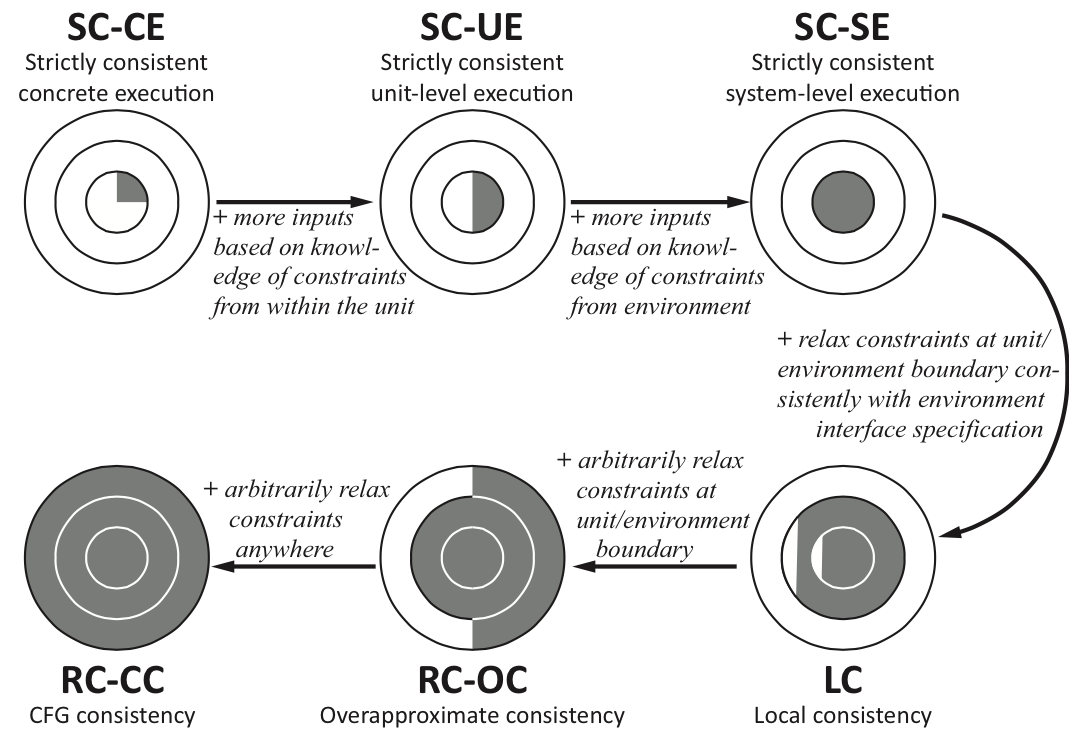
\includegraphics[width=3in]{s2e-consistency-models.png}
\caption{S2E Consistency Models \cite{s2e}}
\label{s2e-cm}
\end{figure}

OUTLINE:

\begin{itemize}
\item Symbolic Execution: KLEE, SAGE, DART, Execution Synthesis
	what Symbolic Execution is?
\item Static Analysis: <insert paper here>
\item Performance vs. Accuracy tradeoff: <insert paper here>
\end{itemize}


\section{Approach}
 research methodology or approach taken in the project
 \begin{itemize}
 \subsection{Sanity Check}
\item Write a few short (< 100 LOC) dummy programs with different bugs (e.g., null pointer dereference, divide by zero, buffer overflow, etc.) to ensure that S2E can catch these bugs before evaluating larger programs - determine coverage of the consistency models before starting.
 \subsection{Dataset}
 \item Select three programs: (1) Web server like apache - lots of network usage (syscalls), (2) Database like SQLlite - lots of file i/o (syscalls), (3) Graphics editing software like Inkscape - lots of computation (not many syscalls expected)
 \subsection{Ground Truth}
\item Look at bug reports for current (or older) versions of these programs to determine what bugs we expect S2E to find (?ground truth?-ish) and evaluate whether we should inject our own bugs. 
 \subsection{Measurement}
\item Use a script or something to get the time of execution start to bug finding (somehow) - check if S2E does logging already (in that case we can just check what time that was added or whatever). Also need to write a script which cuts off S2E after certain time units. 
\end{itemize}

\section{Status}
 current status of implementation
 \begin{itemize}
\item Currently in preparatory phase
\item We have built S2E and tested it on a sample application
\item Gathering dataset, looking at bug reports for each application
\item ~~~ Wrote dummy programs with bugs to ensure the consistency models catch these bugs (sanity check) 
\end{itemize}

\section{Evaluation}
 description of experiments that will be performed
 \begin{itemize}
\item Per consistency model:
Using script described above we will run each of the three applications for different ?time units? (e.g., one hour cutoff, two hour, ?., five hour) and record results (hopefully S2E has a log?..)
\item Analyze bugs caught, comparing them to the ?ground truth? determined previously - this will affect accuracy (false negatives)
\item Depending on the number of bugs caught, manually analyze the source code to determine whether there was an actual bug - also accuracy (false positives) 
\item Create a performance accuracy tradeoff graphs per consistency model. X axis = different ?time units?, Y axis = number (or percentage, etc.) of FPs and FNs (two data lines).
\end{itemize}



% conference papers do not normally have an appendix


% use section* for acknowledgement
%\section*{Acknowledgment}


%The authors would like to thank...





% trigger a \newpage just before the given reference
% number - used to balance the columns on the last page
% adjust value as needed - may need to be readjusted if
% the document is modified later
%\IEEEtriggeratref{8}
% The "triggered" command can be changed if desired:
%\IEEEtriggercmd{\enlargethispage{-5in}}

% references section

% can use a bibliography generated by BibTeX as a .bbl file
% BibTeX documentation can be easily obtained at:
% http://www.ctan.org/tex-archive/biblio/bibtex/contrib/doc/
% The IEEEtran BibTeX style support page is at:
% http://www.michaelshell.org/tex/ieeetran/bibtex/
%\bibliographystyle{IEEEtran}
% argument is your BibTeX string definitions and bibliography database(s)
%\bibliography{IEEEabrv,../bib/paper}
%
% <OR> manually copy in the resultant .bbl file
% set second argument of \begin to the number of references
% (used to reserve space for the reference number labels box)
\begin{thebibliography}{1}

%\bibitem{s2e}
%V.~Chipounov, V.~Georgescu, C.~Zamfir, and G.~Candea.
%\emph{Selective symbolic execution}. In Workshop on Hot Topics
%in Dependable Systems, 2009.
%
%\bibitem{klee}
%C.~Cadar, D.~Dunbar, and D.~R. Engler, \emph{KLEE: 
%Unassisted and automatic generation of high-coverage tests 
%for complex systems programs}. In Symp. on Operating Systems
%Design and Implementation, 2008.

\bibitem{s2e}
CHIPOUNOV, V., GEORGESCU, V., ZAMFIR, C., AND CANDEA, G
Selective symbolic execution. In Workshop on Hot Topics
in Dependable Systems, 2009.

\bibitem{klee}
CADAR, C., DUNBAR, AND ENGLER, D.R. 
KLEE: Unassisted and automatic generation of high-coverage tests 
for complex systems programs. In Symp. on Operating Systems
Design and Implementation, 2008.

\bibitem{cute}
SEN, K., MARINOV, D., AND AGHA, G. CUTE: A concolic unit testing engine for C. In In 5th joint meeting of the European Software Engineering Conference and ACM Symposium on the Foundations of Software Engineering (ESEC/FSE 2005).

\bibitem{RWset}
BOONSTOPPEL, P., CADAR, C., AND ENGLER, D. RWset: At- tacking path explosion in constraint-based test generation. In Proceedings of Tools and Algorithms for the Construction and Analysis of Systems (TACAS 2008).

\bibitem{vul-signature}
BRUMLEY, D., NEWSOME, J., SONG, D., WANG, H., AND JHA, S. Towards automatic generation of vulnerability-based sig- natures. In Proceedings of the 2006 IEEE Symposium on Security and Privacy (IEEE S\&P 2006).

\bibitem{system-crash}
CADAR, C., AND ENGLER, D. Execution generated test cases: How to make systems code crash itself. In Proceedings of the 12th International SPIN Workshop on Model Checking of Soft- ware (SPIN 2005).

\bibitem{exe}
CADAR, C., GANESH, V., PAWLOWSKI, P., DILL, D., AND ENGLER, D. EXE: Automatically generating inputs of death. In Proceedings of the 13th ACM Conference on Computer and Communications Security (CCS 2006).

\bibitem{bad-input}
COSTA, M., CASTRO, M., ZHOU, L., ZHANG, L., AND PEINADO, M. Bouncer: Securing software by blocking bad input. In Proceedings of the 21th ACM Symposium on Operating Systems Principles (SOSP 2007).

\bibitem{end-to-end}
COSTA, M., CROWCROFT, J., CASTRO, M., ROWSTRON, A., ZHOU, L., ZHANG, L., AND BARHAM, P. Vigilante: end-to-end containment of Internet worms. In Proceedings of the 20th ACM Symposium on Operating Systems Principles (SOSP 2005).

\bibitem{dyn-test}
EMMI, M., MAJUMDAR, R., AND SEN, K. Dynamic test input generation for database applications. In International Symposium on Software Testing and Analysis (ISSTA 2007).

\bibitem{compositional-test}
GODEFROID, P. Compositional dynamic test generation. In Proceedings of the 34th Symposium on Principles of Programming Languages (POPL 2007).

\bibitem{dart}
GODEFROID, P., KLARLUND, N., AND SEN, K. DART: Directed automated random testing. In Proceedings of the Conference on Programming Language Design and Implementation (PLDI 2005).

\bibitem{sage}
GODEFROID, P., LEVIN, M. Y., AND MOLNAR, D. Automated whitebox fuzz testing. In Proceedings of Network and Distributed Systems Security (NDSS 2008).

\bibitem{disassembly}
SCHWARZ, B., DEBRAY, S., AND ANDREWS, G. Disassembly of executable code revisited. In Working Conf. on Reverse Engineering, 2002.

\bibitem{saturn}
DIILLIG, I., DILLIG, T., AND ALKEN, A. Sound, complete and scalable path- sensitive analysis. In Conf. on Programming Language Design and Implementation, 2008.

\bibitem{bddbddb}
LAM, M. S., WHALEY, J., LIVSHITS, V. B., MARTIN, M. C., AVOTS, D., CARBIN, M., AND UNKEL, C. Context-sensitive program analysis as
database queries. In Symp. on Principles of Database Systems, 2005.


\end{thebibliography}




% that's all folks
\end{document}


